\documentclass{standalone}
\usepackage{tikz}
\usetikzlibrary{patterns, positioning}


\begin{document}
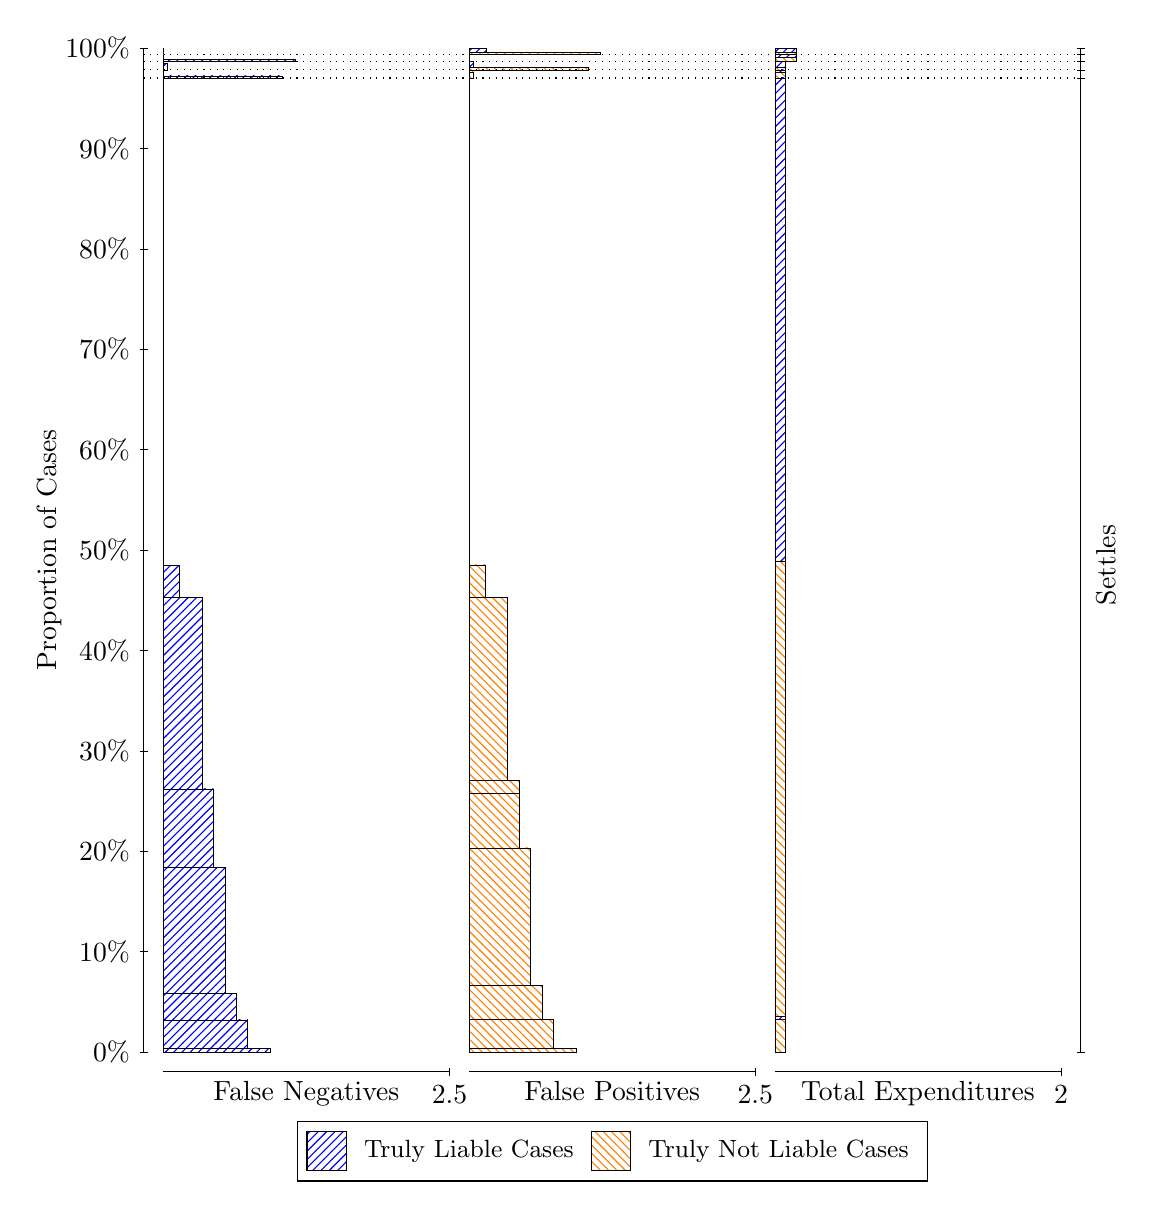
\begin{tikzpicture}
\draw[black, very thin] (1.5,1.75) -- (1.5,14.5);
\node[rotate=90, text=black, anchor=center] at (0.3, 8.125) {Proportion of Cases};
\draw[black, very thin] (1.45,1.75) -- (1.55,1.75);
\node[text=black, anchor=east] at (1.45, 1.75) {0\%};
\draw[black, very thin] (1.45,3.025) -- (1.55,3.025);
\node[text=black, anchor=east] at (1.45, 3.025) {10\%};
\draw[black, very thin] (1.45,4.3) -- (1.55,4.3);
\node[text=black, anchor=east] at (1.45, 4.3) {20\%};
\draw[black, very thin] (1.45,5.575) -- (1.55,5.575);
\node[text=black, anchor=east] at (1.45, 5.575) {30\%};
\draw[black, very thin] (1.45,6.85) -- (1.55,6.85);
\node[text=black, anchor=east] at (1.45, 6.85) {40\%};
\draw[black, very thin] (1.45,8.125) -- (1.55,8.125);
\node[text=black, anchor=east] at (1.45, 8.125) {50\%};
\draw[black, very thin] (1.45,9.4) -- (1.55,9.4);
\node[text=black, anchor=east] at (1.45, 9.4) {60\%};
\draw[black, very thin] (1.45,10.675) -- (1.55,10.675);
\node[text=black, anchor=east] at (1.45, 10.675) {70\%};
\draw[black, very thin] (1.45,11.95) -- (1.55,11.95);
\node[text=black, anchor=east] at (1.45, 11.95) {80\%};
\draw[black, very thin] (1.45,13.225) -- (1.55,13.225);
\node[text=black, anchor=east] at (1.45, 13.225) {90\%};
\draw[black, very thin] (1.45,14.5) -- (1.55,14.5);
\node[text=black, anchor=east] at (1.45, 14.5) {100\%};

\draw[black, very thin] (13.4,1.75) -- (13.4,14.5);
\draw[black, very thin] (13.35,1.75) -- (13.45,1.75);
\node[anchor=west] at (13.35, 1.75) {};
\draw[black, very thin] (13.35,14.12) -- (13.45,14.12);
\node[anchor=west] at (13.35, 14.12) {};
\draw[black, very thin] (13.35,14.222) -- (13.45,14.222);
\node[anchor=west] at (13.35, 14.222) {};
\draw[black, very thin] (13.35,14.33) -- (13.45,14.33);
\node[anchor=west] at (13.35, 14.33) {};
\draw[black, very thin] (13.35,14.415) -- (13.45,14.415);
\node[anchor=west] at (13.35, 14.415) {};
\draw[black, very thin] (13.35,14.5) -- (13.45,14.5);
\node[anchor=west] at (13.35, 14.5) {};

\draw[black, very thin, pattern color=blue, pattern=north east lines] (1.75,1.75) rectangle (3.1125,1.7942);
\draw[black, very thin, pattern color=blue, pattern=north east lines] (1.75,1.7942) rectangle (2.8218,2.1565);
\draw[black, very thin, pattern color=blue, pattern=north east lines] (1.75,2.1565) rectangle (2.6765,2.4924);
\draw[black, very thin, pattern color=blue, pattern=north east lines] (1.75,2.4924) rectangle (2.5312,4.0913);
\draw[black, very thin, pattern color=blue, pattern=north east lines] (1.75,4.0913) rectangle (2.3858,5.0913);
\draw[black, very thin, pattern color=blue, pattern=north east lines] (1.75,5.0913) rectangle (2.2405,7.5236);
\draw[black, very thin, pattern color=blue, pattern=north east lines] (1.75,7.5236) rectangle (1.9498,7.9342);
\draw[black, very thin, pattern color=orange, pattern=north west lines] (1.75,7.9342) rectangle (1.75,14.12);
\draw[black, very thin, pattern color=blue, pattern=north east lines] (1.75,14.12) rectangle (3.2578,14.146);
\draw[black, very thin, pattern color=orange, pattern=north west lines] (1.75,14.146) rectangle (1.75,14.222);
\draw[black, very thin, pattern color=blue, pattern=north east lines] (1.75,14.222) rectangle (1.8045,14.303);
\draw[black, very thin, pattern color=orange, pattern=north west lines] (1.75,14.303) rectangle (1.75,14.33);
\draw[black, very thin, pattern color=blue, pattern=north east lines] (1.75,14.33) rectangle (3.4213,14.359);
\draw[black, very thin, pattern color=orange, pattern=north west lines] (1.75,14.359) rectangle (1.75,14.415);
\draw[black, very thin, pattern color=orange, pattern=north west lines] (1.75,14.415) rectangle (1.75,14.444);
\draw[black, very thin, pattern color=blue, pattern=north east lines] (1.75,14.444) rectangle (1.75,14.5);
\draw[black, very thin, pattern color=orange, pattern=north west lines] (5.6333,1.75) rectangle (6.9958,1.7942);
\draw[black, very thin, pattern color=orange, pattern=north west lines] (5.6333,1.7942) rectangle (6.7052,2.1688);
\draw[black, very thin, pattern color=orange, pattern=north west lines] (5.6333,2.1688) rectangle (6.5598,2.5909);
\draw[black, very thin, pattern color=orange, pattern=north west lines] (5.6333,2.5909) rectangle (6.4145,4.3427);
\draw[black, very thin, pattern color=orange, pattern=north west lines] (5.6333,4.3427) rectangle (6.2692,5.0321);
\draw[black, very thin, pattern color=orange, pattern=north west lines] (5.6333,5.0321) rectangle (6.2692,5.1981);
\draw[black, very thin, pattern color=orange, pattern=north west lines] (5.6333,5.1981) rectangle (6.1238,7.5251);
\draw[black, very thin, pattern color=orange, pattern=north west lines] (5.6333,7.5251) rectangle (5.8332,7.9358);
\draw[black, very thin, pattern color=blue, pattern=north east lines] (5.6333,7.9358) rectangle (5.6333,14.12);
\draw[black, very thin, pattern color=orange, pattern=north west lines] (5.6333,14.12) rectangle (5.6878,14.197);
\draw[black, very thin, pattern color=blue, pattern=north east lines] (5.6333,14.197) rectangle (5.6333,14.222);
\draw[black, very thin, pattern color=orange, pattern=north west lines] (5.6333,14.222) rectangle (7.1412,14.25);
\draw[black, very thin, pattern color=blue, pattern=north east lines] (5.6333,14.25) rectangle (5.6878,14.33);
\draw[black, very thin, pattern color=orange, pattern=north west lines] (5.6333,14.33) rectangle (5.6333,14.386);
\draw[black, very thin, pattern color=blue, pattern=north east lines] (5.6333,14.386) rectangle (5.6333,14.415);
\draw[black, very thin, pattern color=orange, pattern=north west lines] (5.6333,14.415) rectangle (7.3047,14.444);
\draw[black, very thin, pattern color=blue, pattern=north east lines] (5.6333,14.444) rectangle (5.8513,14.5);
\draw[black, very thin, pattern color=orange, pattern=north west lines] (9.5167,1.75) rectangle (9.6529,2.1607);
\draw[black, very thin, pattern color=blue, pattern=north east lines] (9.5167,2.1607) rectangle (9.6529,2.2049);
\draw[black, very thin, pattern color=orange, pattern=north west lines] (9.5167,2.2049) rectangle (9.6529,7.98);
\draw[black, very thin, pattern color=blue, pattern=north east lines] (9.5167,7.98) rectangle (9.6529,14.12);
\draw[black, very thin, pattern color=orange, pattern=north west lines] (9.5167,14.12) rectangle (9.6529,14.197);
\draw[black, very thin, pattern color=blue, pattern=north east lines] (9.5167,14.197) rectangle (9.6529,14.222);
\draw[black, very thin, pattern color=orange, pattern=north west lines] (9.5167,14.222) rectangle (9.6529,14.25);
\draw[black, very thin, pattern color=blue, pattern=north east lines] (9.5167,14.25) rectangle (9.6529,14.33);
\draw[black, very thin, pattern color=orange, pattern=north west lines] (9.5167,14.33) rectangle (9.7892,14.386);
\draw[black, very thin, pattern color=blue, pattern=north east lines] (9.5167,14.386) rectangle (9.7892,14.415);
\draw[black, very thin, pattern color=orange, pattern=north west lines] (9.5167,14.415) rectangle (9.7892,14.444);
\draw[black, very thin, pattern color=blue, pattern=north east lines] (9.5167,14.444) rectangle (9.7892,14.5);
\draw[black, dotted] (1.5,14.12) -- (13.4,14.12);
\draw[black, dotted] (1.5,14.222) -- (13.4,14.222);
\draw[black, dotted] (1.5,14.33) -- (13.4,14.33);
\draw[black, dotted] (1.5,14.415) -- (13.4,14.415);
\draw[black, very thin] (1.75,1.5) -- (5.3833,1.5);
\node[text=black, anchor=north] at (3.5667, 1.5) {False Negatives};
\draw[black, very thin] (5.3833,1.45) -- (5.3833,1.55);
\node[text=black, anchor=north] at (5.3833, 1.45) {2.5};

\draw[black, very thin] (5.6333,1.5) -- (9.2667,1.5);
\node[text=black, anchor=north] at (7.45, 1.5) {False Positives};
\draw[black, very thin] (9.2667,1.45) -- (9.2667,1.55);
\node[text=black, anchor=north] at (9.2667, 1.45) {2.5};

\draw[black, very thin] (9.5167,1.5) -- (13.15,1.5);
\node[text=black, anchor=north] at (11.333, 1.5) {Total Expenditures};
\draw[black, very thin] (13.15,1.45) -- (13.15,1.55);
\node[text=black, anchor=north] at (13.15, 1.45) {2};

\node[text=black, centered, rotate=90] at (13.72, 7.935) {Settles};





\draw (7.449999999999999,1.5) node[draw=none] (baseCoordinate) {};
\begin{scope}[align=center]
        \matrix[scale=0.5, draw=black, below=0.5cm of baseCoordinate, nodes={draw}, column sep=0.1cm]{
            \node[rectangle, draw, minimum width=0.5cm, minimum height=0.5cm, pattern color=blue, pattern=north east lines] {}; &
            \node[draw=none, font=\small, text=black] (B) {Truly Liable Cases}; &
            \node[rectangle, draw, minimum width=0.5cm, minimum height=0.5cm, pattern color=orange, pattern=north west lines] {}; &
            \node[draw=none, font=\small, text=black] (B) {Truly Not Liable Cases}; \\
            };
\end{scope}

\end{tikzpicture}
\end{document}